\begin{figure}[!htbp]
\centering
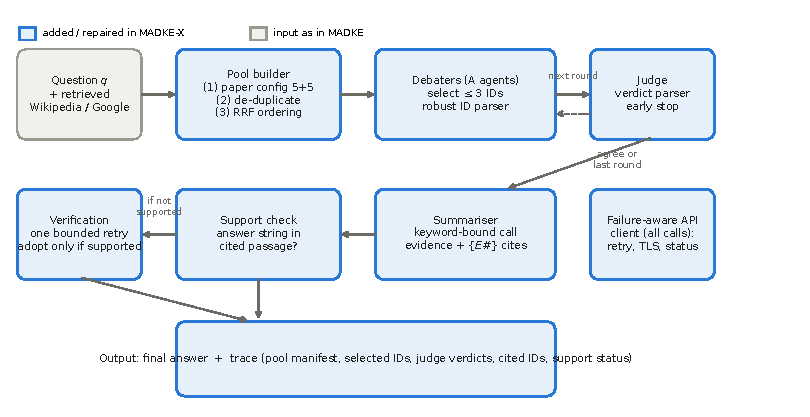
\includegraphics[width=\textwidth]{fig1_architecture}
\caption{MADKE-X architecture. Blue boxes are added or repaired relative to MADKE; the debate control flow is unchanged.}
\label{fig:architecture}
\end{figure}

\section{The proposed method: MADKE-X}
\label{sec:method}

\subsection{Failure-aware interface layer}
Every model call returns an explicit result (ok, error, attempts) from a client with bounded retries and verified TLS; a failed call marks the question as failed instead of letting an error message be scored as an answer. The summariser call is bound by keyword, evidence IDs are parsed by an order-preserving parser that keeps the first three IDs and records everything it ignores (Algorithm~\ref{alg:parse}), the judge verdict is the last bracketed Yes/No, case-insensitive, and the consistency statistics are computed from the stored judge texts including the final round.

\subsection{Evidence governor}
Algorithm~\ref{alg:pool} builds the pool. It uses the paper's configuration (5 Wikipedia + 5 Google passages), where the released code defaulted to 10 + 5, removes passages with identical normalised text, and orders the rest by reciprocal rank fusion of the retrieval rank and a question-only BM25 rank \cite{cormack2009rrf,robertson2009bm25}; no gold answer and no model is used.

\subsection{Decision trace and citations}
Each answer record carries a trace with (i) a pool manifest (index, source, source rank, passage hash), (ii) for every round and agent, the IDs actually delivered, with dropped, ignored and out-of-range IDs, (iii) the judge verdict and how it was parsed, and (iv) the final answer, the evidence IDs it cites as $\{E\#\}$ (a bracket type that cannot collide with the answer brackets) and the result of a support check (Algorithm~\ref{alg:support}). The check detects the \emph{absence} of the answer string from the cited passages; it does not establish entailment.

\begin{algorithm}[!htbp]
\caption{ParseEvidenceIDs}
\label{alg:parse}
\Input{reply $r$, pool size $m$, cap $k{=}3$}
\Output{IDs, not-found flag, audit lists}
$I \leftarrow [\,]$, $O \leftarrow [\,]$, $f \leftarrow \textbf{false}$\;
\ForEach{bracket group $g$ of $r$, in written order}{
  \lIf{$g$ matches no[\_ -]?found (any case)}{$f \leftarrow \textbf{true}$}
  \ElseIf{$g$ is a list of integers}{
    \ForEach{integer $n$ in $g$}{
      \lIf{$n \ge m$}{append $n$ to $O$}
      \lElseIf{$n \notin I$}{append $n$ to $I$}
    }
  }
}
\lIf{$f$}{\textbf{return} $([\,]$, \textbf{true}, ignored$=I$, dropped$=[\,]$, out-of-range$=O)$}
\textbf{return} $(I[{:}k]$, \textbf{false}, $[\,], I[k{:}], O)$\;
\end{algorithm}

\begin{algorithm}[!htbp]
\caption{BuildPool (evidence governor)}
\label{alg:pool}
\Input{question $q$, lists $W$ (Wikipedia), $G$ (Google), $w{=}5$, $g{=}5$, BM25 index $\mathcal{B}$}
\Output{ordered pool $E$}
$E \leftarrow W[{:}w] \,\|\, G[{:}g]$, recording source and source rank $\rho(e)$\;
remove $e$ whose normalised text was already seen\;
rank $E$ by $\mathrm{BM25}_{\mathcal{B}}(q,e)$ to obtain $\beta(e)$\;
\textbf{return} $E$ sorted by decreasing $\dfrac{1}{60+\rho(e)} + \dfrac{1}{60+\beta(e)}$\;
\end{algorithm}

\subsection{Bounded verification (new)}
When the status is not \emph{supported}, the summariser is called once more with the same evidence and an instruction to answer only if a listed passage states the answer, citing it, or otherwise to abstain with \texttt{[Unsupported] \{E-none\}}. The second answer is adopted only if its own support check passes; otherwise the first answer is kept and flagged in the trace. The step adds at most one call per question, never changes an answer that is already supported, and is switched off by default (\texttt{-verify}).

\begin{algorithm}[!htbp]
\caption{SupportCheck}
\label{alg:support}
\Input{answer $a$, cited IDs $C$, pool $E$}
\Output{status}
\lIf{$a = \varepsilon$}{\textbf{return} empty\_answer}
\lIf{$C = \emptyset$}{\textbf{return} no\_citation}
\lIf{normalised $a$ occurs in normalised text of some $E_i$, $i \in C$}{\textbf{return} supported}
\textbf{return} cited\_but\_answer\_not\_found\;
\end{algorithm}

\begin{algorithm}[!htbp]
\caption{MADKE-X (control flow)}
\label{alg:control}
\Input{question $q$, raw retrieval lists, $A$, $R$, flags cite and verify}
\Output{answer, trace}
$E \leftarrow$ BuildPool (Alg.~\ref{alg:pool})\;
\For{$r = 1$ \KwTo $R$}{
  \ForEach{debater $i$}{
    $(I_i) \leftarrow$ ParseEvidenceIDs(select($q$,$E$,$h_i$)) (Alg.~\ref{alg:parse}); $a_i \leftarrow$ answer($q$, $E[I_i]$, $h_i$)\;
  }
  $v \leftarrow$ ParseJudgeVerdict(judge($q$, $a_1..a_A$))\;
  \lIf{any call failed}{mark question failed; \textbf{break}}
  \If{$v = $ yes \textbf{or} $r = R$}{
    $s \leftarrow$ summarise($q$, $a_{1..A}$, $E[\cup I_i]$) with $\{E\#\}$ citations\;
    $c \leftarrow$ SupportCheck($s$)\;
    \If{verify \textbf{and} $c \neq$ supported}{
      $s' \leftarrow$ summarise with verification instruction; adopt $s'$ iff SupportCheck($s'$) $=$ supported\;
    }
    \textbf{break}\;
  }
}
\textbf{return} answer, trace\;
\end{algorithm}
